\documentclass[class=article,crop=false]{standalone} \usepackage[margin=1in,headheight=57pt,headsep=0.1in]{geometry}
\usepackage[subpreambles=true]{standalone}
\usepackage{float}
\usepackage[framemethod=TikZ]{mdframed}
\usepackage{fancyhdr}
\usepackage[utf8]{inputenc} % Required for inputting international characters
\usepackage[T1]{fontenc} % Output font encoding for international characters
\usepackage{stix} % Use the STIX fonts
\usepackage{hyperref}
\hbadness=99999

\begin{document}
\subsection{Edit Enemy Form}
This is the form that is opened when you click the "Edit Enemy" (otherwise "Edit Element") button within the Edit Tile form, when the tile is of type "\texttt{enemy\_room}".
\begin{figure}[H]
	\centering
	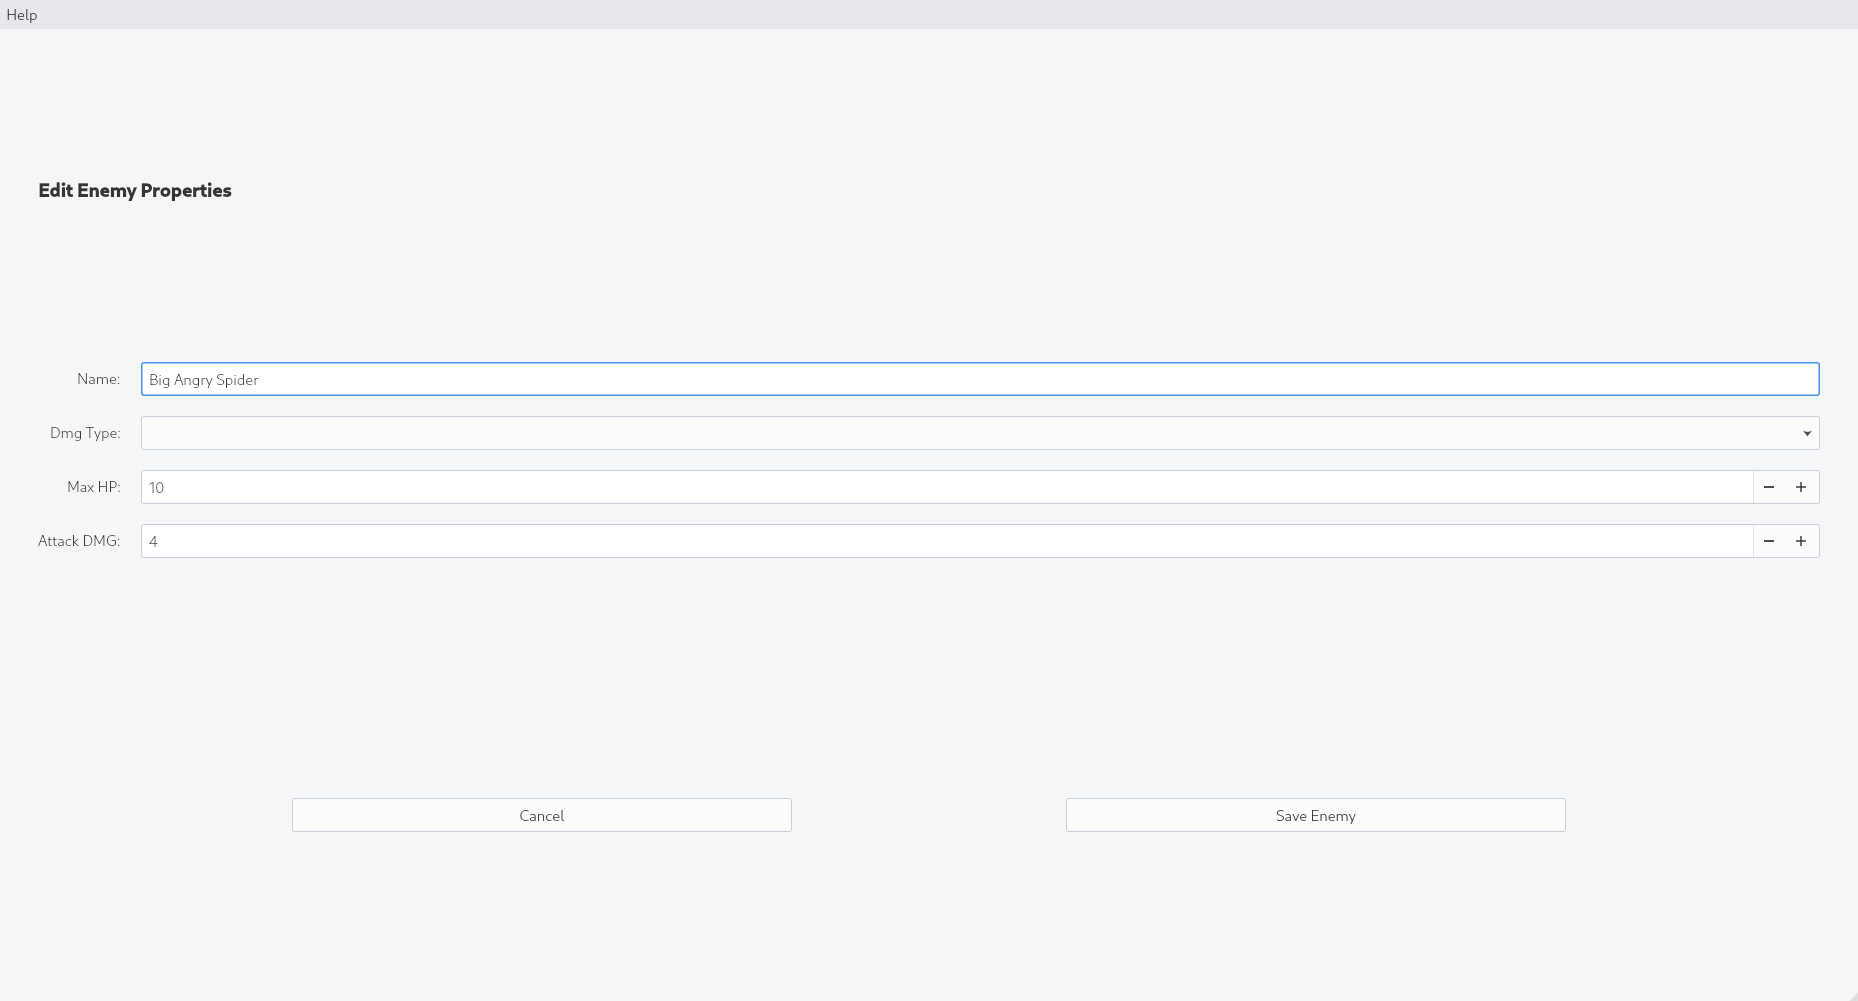
\includegraphics[width=1.0\textwidth]{./editEnemyForm.png}
\end{figure}
\begin{itemize}
	\item Name: this is the name of the enemy within the game, and it will be seen by the player.
	\item Dmg Type: the damage type of the enemy; in more complicated narratives this feature can be used to enrich gameplay. A weapon of a specific damage type interacting with an enemy of the same damage type deals potentially massive damamge.
	\item Max HP: The maximum number of health points carried by the enemy. Note that the player character starts with maximum health at 10 HP.
	\item Attack Dmg: The maximum amount of HP the enemy can detract from the player during one turn of a battle.
	\item Cancel: closes the form without saving changes.
	\item Save Item: closes the form while saving the enemy to the parent Edit Tile form.
\end{itemize}
\end{document}
